% Verze pro jednostranný tisk:
\documentclass[11pt,a4paper]{report}
\usepackage[top=25mm,bottom=25mm,right=25mm,left=30mm,head=12.5mm,foot=12.5mm]{geometry}
\let\openright=\clearpage

%% Definice různých užitečných maker (viz popis uvnitř souboru)
%%% Tento soubor obsahuje definice různých užitečných maker a prostředí %%%
%%% Další makra připisujte sem, ať nepřekáží v ostatních souborech.     %%%

\usepackage[a-2u]{pdfx}     % výsledné PDF bude ve standardu PDF/A-2u

%%% Nastavení pro použití samostatné bibliografické databáze.
\usepackage[
   backend=biber
%  ,style=iso-authoryear
  ,style=authoryear
  ,sortlocale=cs_CZ
  ,bibencoding=UTF8
  %,block=ragged
]{biblatex}
\let\cite\parencite
\bibliography{literatura}

%% Přepneme na českou sazbu, fonty Latin Modern a kódování češtiny
\usepackage[czech]{babel}
\usepackage{lmodern}
\usepackage[T1]{fontenc}
\usepackage{textcomp}
\usepackage[utf8]{inputenc}

%%% Další užitečné balíčky (jsou součástí běžných distribucí LaTeXu)
\usepackage{amsmath}        % rozšíření pro sazbu matematiky
\usepackage{amsfonts}       % matematické fonty
\usepackage{amsthm}         % sazba vět, definic apod.
\usepackage{bm}             % tučné symboly (příkaz \bm)
\usepackage{graphicx}       % vkládání obrázků
\usepackage{fancyvrb}       % vylepšené prostředí pro strojové písmo
\usepackage{fancyhdr}       % prostředí pohodlnější nastavení hlavy a paty stránek
\usepackage{icomma}         % inteligetní čárka v matematickém módu
\usepackage{dcolumn}        % lepší zarovnání sloupců v tabulkách
\usepackage{booktabs}       % lepší vodorovné linky v tabulkách
\makeatletter
\@ifpackageloaded{xcolor}{
   \@ifpackagewith{xcolor}{usenames}{}{\PassOptionsToPackage{usenames}{xcolor}}
  }{\usepackage[usenames]{xcolor}} % barevná sazba
\makeatother
\usepackage{multicol}       % práce s více sloupci na stránce
\usepackage{caption}
\usepackage{enumitem}
\setlist[itemize]{noitemsep, topsep=0pt, partopsep=0pt}
\setlist[enumerate]{noitemsep, topsep=0pt, partopsep=0pt}
\setlist[description]{noitemsep, topsep=0pt, partopsep=0pt}

\usepackage{tocloft}
\setlength\cftparskip{0pt}
\setlength\cftbeforechapskip{1.5ex}
\setlength\cftfigindent{0pt}
\setlength\cfttabindent{0pt}
\setlength\cftbeforeloftitleskip{0pt}
\setlength\cftbeforelottitleskip{0pt}
\setlength\cftbeforetoctitleskip{0pt}
\renewcommand{\cftlottitlefont}{\Huge\bfseries\sffamily}
\renewcommand{\cftloftitlefont}{\Huge\bfseries\sffamily}
\renewcommand{\cfttoctitlefont}{\Huge\bfseries\sffamily}

% vyznaceni odstavcu
\parindent=0pt
\parskip=11pt

% zakaz vdov a sirotku - jednoradkovych pocatku ci koncu odstavcu na prechodu mezi strankami
\clubpenalty=1000
\widowpenalty=1000
\displaywidowpenalty=1000

% nastaveni radkovani
\renewcommand{\baselinestretch}{1.20}

% nastaveni pro nadpisy - tucne a bezpatkove
\usepackage{sectsty}    
\allsectionsfont{\sffamily}

% nastavení hlavy a paty stránek
\renewcommand{\footrulewidth}{.5pt}
\fancypagestyle{plain}{%
\fancyhf{} % clear all header and footer fields
\fancyfoot[C]{\thepage} %% [RO,LE] vyvolalo warning, odstraněno
\renewcommand{\headrulewidth}{0pt}
\renewcommand{\footrulewidth}{0.5pt}}

% Tato makra přesvědčují mírně ošklivým trikem LaTeX, aby hlavičky kapitol
% sázel příčetněji a nevynechával nad nimi spoustu místa. Směle ignorujte.
\makeatletter
\def\@makechapterhead#1{
  {\parindent \z@ \raggedright \sffamily
   \Huge\bfseries \thechapter. #1
   \par\nobreak
   \vskip 20\p@
}}
\def\@makeschapterhead#1{
  {\parindent \z@ \raggedright \sffamily
   \Huge\bfseries #1
   \par\nobreak
   \vskip 20\p@
}}
\makeatother

% Trochu volnější nastavení dělení slov, než je default.
\lefthyphenmin=2
\righthyphenmin=2

% Zapne černé "slimáky" na koncích řádků, které přetekly, abychom si
% jich lépe všimli.
\overfullrule=1mm

%% Balíček hyperref, kterým jdou vyrábět klikací odkazy v PDF,
%% ale hlavně ho používáme k uložení metadat do PDF (včetně obsahu).
%% Většinu nastavítek přednastaví balíček pdfx.
\hypersetup{unicode}
\hypersetup{breaklinks=true}
\hypersetup{hidelinks}
\hypersetup{
    colorlinks = true,
    allcolors = black,
    urlcolor = blue
}

%%% Prostředí pro sazbu kódu, případně vstupu/výstupu počítačových
%%% programů. (Vyžaduje balíček fancyvrb -- fancy verbatim.)

\DefineVerbatimEnvironment{code}{Verbatim}{fontsize=\small, frame=single}

%%% Použití zkratek
\usepackage{acronym}
\usepackage{csquotes}

%%% Zabrání rozdělení paragrafů mezi stránkami
\widowpenalties 1 10000
\raggedbottom

\usepackage{float}
\usepackage{mathtools}
\DeclarePairedDelimiter{\ceil}{\lceil}{\rceil}

\graphicspath{ {./img/} }
\overfullrule=0pt


%%% Údaje o práci
% Název práce v jazyce práce (přesně podle zadání)
\def\NazevPrace{Modely logistické regrese v oblasti esportových dat}

% Typ práce
\def\TypPrace{BAKALÁŘSKÁ PRÁCE}


% Jméno autora
\def\AutorPrace{Michal Lauer}

% Rok odevzdání. měsíc (slovně)
\def\DatumOdevzdani{Duben 2022}

% Vedoucí práce: Jméno a příjmení s~tituly
\def\Vedouci{Ing. Zdeněk Šulc, Ph.D.}

% Studijní program a obor
\def\StudijniProgram{Aplikovaná informatika}
\def\StudijniObor{Aplikovaná informatika}

% Text čestného prohlášení pro MUŽE pro bakalářskou práci
\def\Prohlaseni{Prohlašuji, že jsem bakalářskou práci \textit{\NazevPrace} vypracoval samostatně za použití v práci uvedených pramenů a literatury.}

% Nepovinné poděkování (vedoucímu práce, konzultantovi, tomu, kdo
% zapůjčil software, literaturu apod.)
\def\Podekovani{%
Rád bych poděkoval panu doktorovi Zdenku Šulcovi, který mou bakalářskou práci podpořil, i přes odlišný studijní obor.
Dále děkuji autorům knih, jmenovitě ... , za poskytnutou příležitost se ve logistických modelech zlepšit. Bez nich by se práce psala velmi složitě.
}

% Abstrakt (doporučený rozsah cca 150-250 slov; nejedná se o zadání práce)
\def\Abstrakt{%
Práce se zabývá predikcí výsledku esportových zápasů dle několika proměnných. V prvním rámci bakalářské práce je v krátkosti představen esport a problematika, kterou se práce zabývá. Dále jsou zde
představeny důležité termíny a pojmy, které jsou klíčkové ke správné interpretaci výsledků. V druhé části, která se zabává teorií, jsou představeny metody k popisu dat, modely, a hodnocení kvality modelů. V poslední části
jsou metody  použity v praxi. Nejprve je představen dataset a jeho proměnné. Z proměnných je vybráno pouze několik hlavních prediktorů, které jsou následně použity k výsledné predikci. Dále se zde nachází
popis prediktorů a pomocí grafů a slovní interpretace. V závěru je zde sestaven multivariabilní logistický regresní model, který předpovídá výsledek zápasů. Ten je vyhodnocen vyhodnocen pomocí již zmínených statistik.    
}
\def\AbstraktEN{%
-- Bude přeložen po odsouhlasení abstraktu v češtině
}

% 3 až 5 klíčových slov (doporučeno)
\def\KlicovaSlova{klíčové slovo, další pojem, jiný důležitý termín, a ještě jeden}
\def\KlicovaSlovaEN{keyword, important term, another topic, and another one}

%% Titulní strana a různé povinné informační strany
\begin{document}
%%% Titulní strana práce a další povinné informační strany

%%% Titulní strana práce

\pagestyle{empty}
\hypersetup{pageanchor=false}

\begin{center}
\Huge\sffamily
Vysoká škola ekonomická v Praze\\
Fakulta informatiky a statistiky

\vspace{\stretch{1}}


\includegraphics[width=.3\textwidth]{img/logo-FIS}

\vspace{\stretch{2}}

\bfseries\NazevPrace

\vspace{8mm}
\mdseries\TypPrace

\vspace{8mm}
\large
\begin{tabular}{rl}
Studijní program: & \StudijniProgram \\
\noalign{\vspace{2mm}}
Studijní obor: & \StudijniObor \\
\end{tabular}

\vspace{\stretch{8}}

\begin{tabular}{rl}
Autor: & \AutorPrace \\
\noalign{\vspace{2mm}}
Vedoucí práce: & \Vedouci \\
\end{tabular}

\vspace{8mm}
Praha, \DatumOdevzdani
\end{center}


\openright

%%% Strana s čestným prohlášením k bakalářské práci

\hypersetup{pageanchor=true}
\pagestyle{plain}
\cleardoublepage
\vspace*{\fill}
\section*{Prohlášení}
\noindent
\Prohlaseni

\vspace{2cm}
\noindent
V Praze dne DD. Dubna 2021
\hfill%
\begin{minipage}[t]{.5\textwidth}%
\begin{center}
\dotfill\\
Podpis studenta
\end{center}
\end{minipage}
\vspace{1cm}

%%% Poděkování
\openright
\vspace*{\fill}
\section*{Poděkování}
\noindent
\Podekovani
\vspace{1cm}


%%% Povinná informační strana bakalářské práce
\openright
\section*{Abstrakt}
\noindent
\Abstrakt
\subsection*{Klíčová slova}
\noindent
\KlicovaSlova

\bigskip\bigskip\bigskip
\section*{Abstract}
\noindent
\AbstraktEN
\subsection*{Keywords}
\noindent
\KlicovaSlovaEN

\openright


%%% Strana s automaticky generovaným obsahem bakalářské práce
\setcounter{tocdepth}{2}
\tableofcontents

%%% Obrázky v bakalářské práci
\openright
\listoffigures

%%% Tabulky v bakalářské práci (opět nemusí být nutné uvádět)
\clearpage
\listoftables

%%% Použité zkratky v bakalářské práci (opět nemusí být nutné uvádět)
\chapter*{Seznam použitých zkratek}
\addcontentsline{toc}{chapter}{Seznam použitých zkratek}

\begin{acronym}
    %% esport tituly
    \acro{CSGO}{Coutner-Strike: Global Offensive}
    %% esport žánry
    \acro{BR}{Battle Royale}
    \acro{MOBA}{Multiplayer Online Battle Arena}
    \acro{FPS}{First-Person Shooter}
    %% ostatní
    \acro{TGNS}{Twin Galaxies National Scoreboard}
\end{acronym}


\pagestyle{fancy}
%%% Jednotlivé kapitoly práce jsou pro přehlednost uloženy v samostatných souborech
\chapter*{Úvod}
\addcontentsline{toc}{chapter}{Úvod}
Esport je jedno z nejrychleji rostoucích odvětví v dnešní době. V roce 2021 se jeho tržní hodnota pohybovala kolem jedné miliardy dolarů - skoro
50\% nárůst oproti roku 2020. Dle portálu statista.com lze předpovídat, že v roce 2024 esport překročí hodnotu 1,5 miliardy dolarů \cite{Gough2021}.
Dalo by se spekulovat, že za takový velký nárůst je zodpovědná aktuální pandemie. Většina populace, hlavně ta mladší, je nucena zůstat doma. Toto otevřelo dveře
se s esportem přirozeně seznámit a nějakým způsobem se ho účastnit \textit{(online divák, soutěžící, organizátor, fanoušek...)}. Esport je vlastně sport,
akorát s počítačovými hrami. Hrají se různé kategorie her - střílečky \textit{(\ac{CS:GO}, Valorant)}, arény \textit{(\ac{LoL})}, či karetní hry
\textit{(\ac{HS})}.

Toto téma jsem si zvolil hlavně kvůli tomu, že se o oblast zajímám od mého mládí. Když jsem si vybíral téma na bakalářskou práci,
chtěl jsem propojit statistiku s něčím, co mě baví a naplňuje - toto je ideální kombinace. Zároveň bylo mím cílem vytvořit práci, která bude v dnešní době relevantní.
Zvolené téma je dle mého názoru velmi aktuální, avšak ne pro širokou veřejnost, nýbrž pouze pro lidi, co se o zajímají o esport či sázení.
Podobné logistické modely, avšak velmi složitější, mohou totiž sloužit například k vyhodnocení sázkových kurzů. Esport, tak jak klasický sport, je se sázením propojen. 

Finální cíl práce je vytvořit logistický model, který předpovídá výsledek zápasů. Tento model je vyhodnocen různými klasifikacemi pro vyhodnocení kvality.
Práce také popisuje grafické metody vizualizace dat a teorii k tvorbě a vyhodnocení logistických modelů. Také zde najdeme popis datového souboru a postup,
jakým byli vybráni nejvýznamnější prediktory - ať už statisticky, či čistě ze znalosti esportu. 

%%% Fiktivní kapitola s ukázkami sazby

\chapter{Nápověda k~sazbě}

\section{Úprava práce}

Vlastní text práce je uspořádaný hierarchicky do kapitol a podkapitol,
každá kapitola začíná na nové straně. Text je zarovnán do bloku. Nový odstavec
se obvykle odděluje malou vertikální mezerou a odsazením prvního řádku. Grafická
úprava má být v~celém textu jednotná.

Zkratky použité v textu musí být vysvětleny vždy u prvního výskytu zkratky (v~závorce nebo
v poznámce pod čarou, jde-li o složitější vysvětlení pojmu či zkratky). Pokud je zkratek
více, připojuje se seznam použitých zkratek, včetně jejich vysvětlení a/nebo odkazů
na definici.

Delší převzatý text jiného autora je nutné vymezit uvozovkami nebo jinak vyznačit a řádně
citovat.

\section{Jednoduché příklady}

Mezi číslo a jednotku patří úzká mezera: šířka stránky A4 činí $210\,\rm mm$, což si
pamatuje pouze $5\,\%$ autorů. Pokud ale údaj slouží jako přívlastek, mezeru vynecháváme:
$25\rm mm$ okraj, $95\%$ interval spolehlivosti.

Rozlišujeme různé druhy pomlček:
červeno-černý (krátká pomlčka),
strana 16--22 (střední),
$45-44$ (matematické minus),
a~toto je --- jak se asi dalo čekat --- vložená věta ohraničená dlouhými pomlčkami.

V~českém textu se používají \uv{české} uvozovky, nikoliv ``anglické''.

% V tomto odstavci se vlnka zviditelňuje
{
\def~{{\tt\char126}}
Na některých místech je potřeba zabránit lámání řádku (v~\TeX{}u značíme vlnovkou):
u~před\-lo\-žek (neslabičnych, nebo obecně jednopísmenných), vrchol~$v$, před $k$~kroky,
a~proto, \dots{} obecně kdekoliv, kde by při rozlomení čtenář \uv{ško\-brt\-nul}.
}

%%% Fiktivní kapitola s ukázkami tabulek, obrázků a kódu

\chapter{Tabulky, obrázky, programy}

Používání tabulek a grafů/obrázků v~odborném textu má některá společná pravidla a~některá specifická. Tabulky a grafy/obrázky neuvádíme přímo do textu, ale umístíme je buď na samostatné stránky nebo na vyhrazené místo v~horní nebo dolní části běžných stránek. \LaTeX\ se o~umístění plovoucích grafů a tabulek postará automaticky.

Grafy/obrázky a tabulky se číslují a jsou vybaveny legendou. Legenda má popisovat obsah grafu či tabulky tak podrobně, aby jim čtenář rozuměl bez důkladného studování textu práce.

Na tabulku a graf/obrázek musí být v~textu číselný odkaz (lze důrazně doporučit dynamický mechanismus křížových referencí, jený je součástí \LaTeX u). Na příslušném místě textu pak shrneme ty nejdůležitější závěry, které lze z~tabulky či grafu učinit. Text by měl být čitelný a srozumitelný i~bez prohlížení tabulek a grafů a tabulky a grafy by měly být srozumitelné i~bez podrobné četby textu.

Na tabulky a grafy odkazujeme pokud možno nepřímo v~průběhu běžného
toku textu; místo \emph{\uv{Tabulka~\ref{tab03:Nejaka} ukazuje, že
    muži jsou v~průměru o~$9,9\,\rm kg$ těžší než ženy}} raději napíšeme
\emph{\uv{Muži jsou o~$9,9\,\rm kg$ těžší než ženy (viz
    tab.~\ref{tab03:Nejaka})}}.

\section{Tabulky}

\begin{table}[htbp!]

\centering
%%% Tabulka používá následující balíčky:
%%%   - booktabs (\toprule, \midrule, \bottomrule)
%%%   - dcolumn (typ sloupce D: vycentrovaná čísla zarovnaná na
%%%     desetinnou čárku
%%%     Všimněte si, že ve zdrojovém kódu jsou desetinné tečky, ale
%%%     tisknou se čárky.

\caption{Maximálně věrohodné odhady v~modelu M.}\label{tab03:Nejaka}
\begin{tabular}{lD{.}{,}{3.2}D{.}{,}{1.2}D{.}{,}{2.3}}
\toprule
               &                & \multicolumn{1}{c}{\textbf{Směrod.}}   &  \\
\textbf{Efekt} & \multicolumn{1}{c}{\textbf{Odhad}} & \multicolumn{1}{c}{\textbf{chyba}$^a$} & \multicolumn{1}{c}{\textbf{P-hodnota}} \\
\midrule
Abs. člen     & -10.01 & 1.01 & \multicolumn{1}{c}{---} \\
Pohlaví (muž) & 9.89   & 5.98 & 0.098 \\
Výška (cm)    & 0.78   & 0.12 & <0.001 \\
\bottomrule
\multicolumn{4}{l}{\footnotesize \textit{Pozn:}$^a$ Směrodatná chyba odhadu metodou Monte Carlo.}
\end{tabular}
\end{table}

U~\textbf{tabulek} se doporučuje dodržovat následující pravidla:

\begin{itemize} %% nebo compactitem z balíku paralist
\item Vyhýbat se svislým linkám. Silnějšími vodorovnými linkami
  oddělit tabulku od okolního textu včetně legendy, slabšími
  vodorovnými linkami oddělovat záhlaví sloupců od těla tabulky a
  jednotlivé části tabulky mezi sebou. V~\LaTeX u tuto podobu tabulek
  implementuje balík \texttt{booktabs}. Chceme-li výrazněji oddělit
  některé sloupce od jiných, vložíme mezi ně větší mezeru.
\item Neměnit typ, formát a význam obsahu políček v~tomtéž sloupci
  (není dobré do téhož sloupce zapisovat tu průměr, onde procenta).
\item Neopakovat tentýž obsah políček mnohokrát za sebou. Máme-li
  sloupec \textit{Rozptyl}, který v~prvních deseti řádcích obsahuje
  hodnotu $0,5$ a v~druhých deseti řádcích hodnotu $1,5$, pak tento
  sloupec raději zrušíme a vyřešíme to jinak. Například můžeme tabulku
  rozdělit na dvě nebo do ní vložit popisné řádky, které informují
o~nějaké proměnné hodnotě opakující se v~následujícím oddíle tabulky
  (např. \emph{\uv{Rozptyl${}=0,5$}} a níže \emph{\uv{Rozptyl${}=
      1,5$}}).
\item Čísla v~tabulce zarovnávat na desetinnou čárku.
\item V~tabulce je někdy potřebné používat zkratky, které se jinde
nevyskytují. Tyto zkratky můžeme vysvětlit v~legendě nebo
v~poznámkách pod tabulkou. Poznámky pod tabulkou můžeme využít i
k~podrobnějšímu vysvětlení významu  některých sloupců nebo hodnot.
\end{itemize}


\section{Obrázky}

\begin{figure}[htbp!]\centering
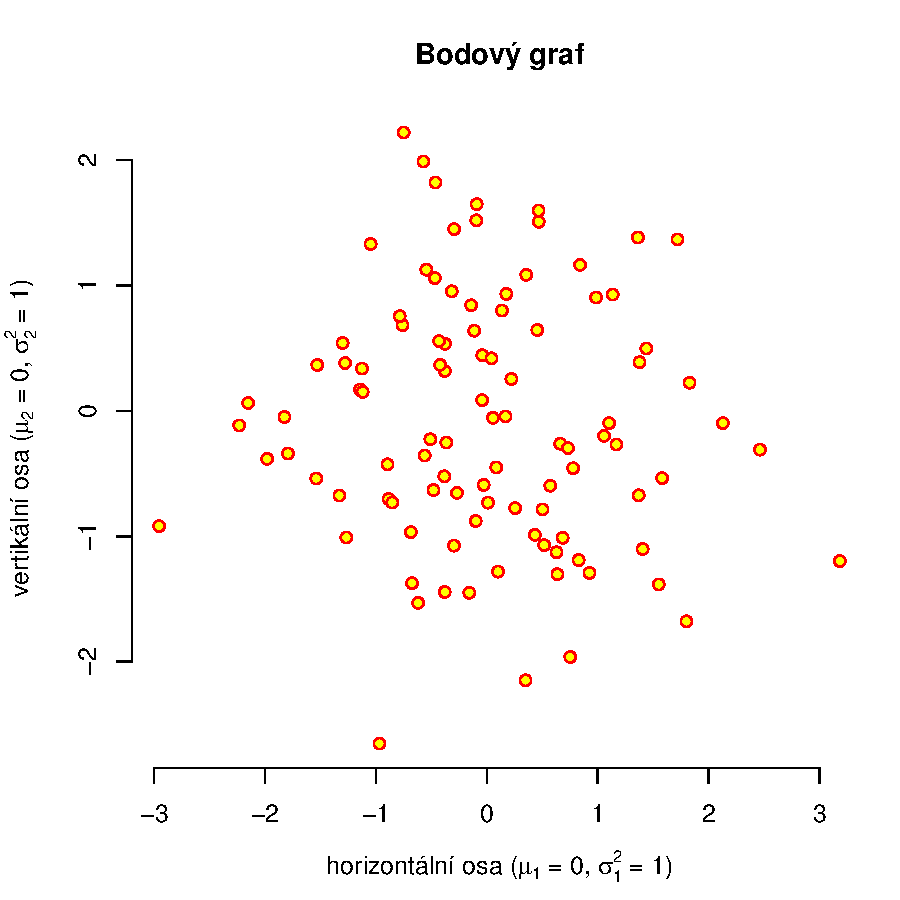
\includegraphics[width=.66\textwidth]{img/ukazka-obr01}
% Příponu není potřeba explicitně uvádět, pdflatex automaticky hledá pdf.
% Rozměry také není nutné uvádět.
\caption{Náhodný výběr z~rozdělení $\mathcal{N}_2(\boldsymbol{0},\,I)$.}
\label{obr03:Nvyber}
\end{figure}

Několik rad týkajících se obrázků a grafů.

\begin{itemize}
\item Graf by měl být vytvořen ve velikosti, v~níž bude použit
  v~práci. Zmenšení příliš velkého grafu vede ke špatné čitelnosti
  popisků.
\item Osy grafu musí být řádně popsány ve stejném jazyce, v~jakém je
  psána práce (absenci diakritiky lze tolerovat). Kreslíme-li graf
  hmotnosti proti výšce, nenecháme na nich popisky \texttt{ht} a
  \texttt{wt}, ale osy popíšeme \emph{Výška [cm]} a~\emph{Hmotnost
    [kg]}. Kreslíme-li graf funkce $h(x)$, popíšeme osy $x$ a $h(x)$.
  Každá osa musí mít jasně určenou škálu.
\item Chceme-li na dvourozměrném grafu vyznačit velké množství bodů,
  dáme pozor, aby se neslily do jednolité černé tmy. Je-li bodů mnoho,
  zmenšíme velikost symbolu, kterým je vykreslujeme, anebo vybereme
  jen malou část bodů, kterou do grafu zaneseme. Grafy, které obsahují
  tisíce bodů, dělají problémy hlavně v~elektronických dokumentech,
  protože výrazně zvětšují velikost souborů.
\item Budeme-li práci tisknout černobíle, vyhneme se používání barev.
  Čáry roz\-li\-šu\-je\-me typem (plná, tečkovaná, čerchovaná,\ldots), plochy
  dostatečně roz\-díl\-ný\-mi intensitami šedé nebo šrafováním. Význam
  jednotlivých typů čar a~ploch vysvětlíme buď v~textové legendě ke
  grafu anebo v~grafické legendě, která je přímo součástí obrázku.
\item Vyhýbejte se bitmapovým obrázkům o~nízkém rozlišení a zejména
  JPEGům (zuby a kompresní artefakty nevypadají na papíře pěkně).
  Lepší je vytvářet obrázky vektorově a vložit do textu jako PDF.
\end{itemize}


\section{Zdrojové kódy}
Algoritmy, výpisy programů a popis interakce s~programy je vhodné odlišit od ostatního textu. Jednou z~možností je použití {\LaTeX}o\-vé\-ho balíčku \texttt{fancyvrb} (fancy verbatim), pomocí něhož je v~souboru \texttt{makra.tex} nadefinováno prostředí \texttt{code}. Pomocí něho lze vytvořit např. následující ukázky.

\begin{code}
> mean(x)
[1] 158.90
> objekt$prumer
[1] 158.90
\end{code}

Jinou vhodnou alternativou je použití balíčku \texttt{listings} a jeho prostředí \texttt{lstlisting}, které je velmi bohatě konfigurovatelné. Příklady:
\begin{itemize}
\item \url{https://en.wikibooks.org/wiki/LaTeX/Source_Code_Listings}
\item \url{https://www.overleaf.com/learn/latex/Code_listing#Using_listings_to_highlight_code}
\end{itemize}


\section{Sazba matematiky}
Proměnné sázíme kurzívou (to \TeX{} v~matematickém módu dělá sám, ale
nezapomínejte na to v~okolním textu a také si matematický mód zapněte).
Názvy funkcí sázíme vzpřímeně. Tedy například:
$\textrm{var} (X) = \textsf{E~} X^2 - \bigl(\textsf{E~} X \bigr)^2$.

Zlomky uvnitř odstavce (třeba $\frac{5}{7}$ nebo $\frac{x+y}{2}$) mohou
být příliš stísněné, takže je lepší sázet jednoduché zlomky s~lomítkem:
$5/7$, $(x+y)/2$.

Možnosti \LaTeX u pro sazbu matematiky jsou sice bohaté, ale je možné, že v některých specifických situacích nebudou postačovat. Proto lze doporučit k použití balíčky American Mathematical Society (AMS). V souboru \texttt{makra.tex} jsou standardně zaváděny balíčky \texttt{amsmath}, \texttt{amsfonts} a \texttt{amsthm}. Pro proniknutí do jejich možností poslouží:
\begin{itemize}
\item Math Extension with AMS\LaTeX\ -- \url{http://ptgmedia.pearsoncmg.com/images/0321173856/samplechapter/kopkach15.pdf}
\item \url{https://www.overleaf.com/learn/latex/Aligning_equations_with_amsmath}
\item Math Mode -- \url{http://tex.loria.fr/general/Voss-Mathmode.pdf}
\item More Math into LaTeX -- \url{http://tug.ctan.org/info/Math_into_LaTeX-4/Short_Course.pdf}
\end{itemize}

%%% Fiktivní kapitola s ukázkami citací

\chapter{Práce s literaturu}

Šablona předpokládá použití bibliografické databáze z důvodu větší flexibility. Použití bibliografické databáze není nutnou podmínkou, lze si vystačit i se standardním prostředím \texttt{thebibliography}. V takovém případě je však zapotřebí provést zásahy do některých souborů, jak je uvedeno dále.

\section{Použití bibliografické databáze}

\begin{enumerate}
\item\textbf{Změna názvu databáze}\\
V šabloně se předpokládá databáze uložená v souboru \texttt{literatura.bib}. Pokud se databáze jmenuje jinak, pak je nutné v souboru \texttt{makra.tex} změnit hodnotu parametru příkazu \verb'\bibliography'.
\item\textbf{Změna citačního stylu}\\
Standardně se citace v textu uvádějí v číselné variantě. Na použití kombinace příjmení a roku lze snadno přepnout změnou v souboru \texttt{makra.tex}, kde se prohodí komentářový znak v parametrech pro balíček \texttt{biblatex}.
\end{enumerate}


\section{Použití prostředí \texttt{thebibliography}}
\begin{enumerate}
\item V souboru \texttt{makra.tex} vymazat na počátku tyto řádky:
\begin{verbatim}
%%% Nastavení pro použití samostatné bibliografické databáze.
\usepackage[
   backend=biber
  ,style=iso-authoryear %iso-numeric
  ,sortlocale=cs_CZ
  ,bibencoding=UTF8
  %,block=ragged
]{biblatex}
\bibliography{literatura}
\end{verbatim}
\item V souboru \texttt{literatura.tex} odstranit řádek s příkazem \verb'\printbibliography' a odstranit příznak komentáře v další části obsahující prostředí \texttt{thebibliography.}
\end{enumerate}


\section{Jak citovat v textu}
\begin{center}
\begin{tabular}{l@{~~$\longrightarrow$~~}l}
\verb|\cite{Cermak2018}|&\cite{Cermak2018}\\
\verb|\cite{Hladik2018,Jasek2018}|&\cite{Hladik2018,Jasek2018}\\
\verb|\cite[kap. 3]{Pecakova2018}|&\cite[kap. 3]{Pecakova2018}\\
\end{tabular}
\end{center}

%%% Fiktivní kapitola s instrukcemi k PDF/A

\chapter{Formát PDF/A}

Elektronická podoba závěrečných
prací musí být odevzdávána ve formátu PDF/A úrovně 1a nebo 2u. To jsou
profily formátu PDF určující, jaké vlastnosti PDF je povoleno používat,
aby byly dokumenty vhodné k~dlouhodobé archivaci a dalšímu automatickému
zpracování. Dále se budeme zabývat úrovní 2u, kterou sázíme \TeX{}em.

Mezi nejdůležitější požadavky PDF/A-2u patří:

\begin{itemize}

\item Všechny fonty musí být zabudovány uvnitř dokumentu. Nejsou přípustné
odkazy na externí fonty (ani na \uv{systémové}, jako je Helvetica nebo Times).

\item Fonty musí obsahovat tabulku ToUnicode, která definuje převod z~kódování
znaků použitého uvnitř fontu to Unicode. Díky tomu je možné z~dokumentu
spolehlivě extrahovat text.

\item Dokument musí obsahovat metadata ve formátu XMP a je-li barevný,
pak také formální specifikaci barevného prostoru.

\end{itemize}

Tato šablona používá balíček {\tt pdfx,} který umí \LaTeX{} nastavit tak,
aby požadavky PDF/A splňoval. Metadata v~XMP se generují automaticky podle
informací v~souboru {\tt prace.xmpdata} (na vygenerovaný soubor se můžete
podívat v~{\tt pdfa.xmpi}).

Správnost PDF/A lze zkontrolovat pomocí on-line validátoru: \url{https://www.pdf-online.com/osa/validate.aspx/}.

Pokud soubor nebude validní, mezi obvyklé příčiny patří používání méně
obvyklých fontů (které se vkládají pouze v~bitmapové podobě a/nebo bez
unicodových tabulek) a vkládání obrázků v~PDF, které samy o~sobě standard
PDF/A nesplňují.

Je pravděpodobné, že se to týká obrázků vytvářených mnoha různými programy.
V~takovém případě se můžete pokusit obrázek do zkonvertovat do PDF/A pomocí
GhostScriptu, například takto:

\begin{verbatim}
        gs -q -dNOPAUSE -dBATCH
           -sDEVICE=pdfwrite -dPDFSETTINGS=/prepress
           -sOutputFile=vystup.pdf vstup.pdf
\end{verbatim}

% \include{...}
% \include{...}
\chapter*{Závěr}
\addcontentsline{toc}{chapter}{Závěr}

Závěr je povinnou částí bakalářské/diplomové práce. Obsahuje shrnutí práce a vyjadřuje se k míře splnění cíle, který byl v práci stanoven, případně shrnuje odpovědi na otázky, které byly položeny v úvodu práce. 

Závěr k diplomové práci musí být propracovanější -- podrobněji to je uvedeno v Náležitostech diplomové práce v rámci Intranetu pro studenty FIS.

Závěr je vnímán jako kapitola (chapter), která začíná na samostatné stránce a která má název Závěr.  Název Závěr se nečísluje. Samotný text závěru je členěn do odstavců.

%%% Seznam použité literatury
%% Toto platí v případě použití samostatné bibliografické databáze
\printbibliography[title={Seznam použité literatury}, heading={bibintoc}, keyword={literatura}]

\printbibliography[title={Seznam elektronických zdrojů}, heading={bibintoc}, keyword={ezdroj}]


%%% Přílohy k bakalářské práci, existují-li. Každá příloha musí být alespoň jednou
%%% odkazována z vlastního textu práce. Přílohy se číslují.
\part*{Přílohy}
\appendix
\chapter{Formulář v plném znění}


\chapter{Zdrojové kódy výpočetních procedur}


% \include{...}
% \include{...}

\end{document}
